\documentclass{article}
\usepackage{graphicx}
\usepackage{parskip}
\usepackage{float}
\usepackage{multicol}
\usepackage{hyperref}

\begin{document}

\begin{center}
    \begin{figure}
        \centering
        
\includegraphics[width = 4cm]{Logo.png}
    \end{figure}
    \par
    02312, 62531, 02314 og 62532.
    \par
    \underline{Development Methods for IT Systems Fall 23}
\end{center}

\hrulefill

\begin{center}
    \LARGE{CDIO 3 Report} \\
    \Large{Group 3}
\end{center}

\hrulefill

\par

\begin{figure} [H]
    
\includegraphics[width=.20\textwidth]{Samin.png}\hfill
    
\includegraphics[width=.20\textwidth]{Daniall.png}\hfill
    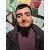
\includegraphics[width=.20\textwidth]{Andrei.png}\hfill
    
\includegraphics[width=.20\textwidth]{Daniel.png}\hfill
    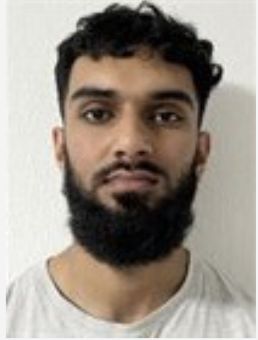
\includegraphics[width=.20\textwidth]{Abdullah.png}
\end{figure}
\begin{multicols}{5}
Chowdhury, \\
Samin \\
S235078
\vfill\null
\columnbreak
Mudasar, \\
Daniall \\
S235070
\vfill\null
\columnbreak
Enache, \\
Andrei \\
S235089
\vfill\null
\columnbreak
Rahimpour, \\
Daniel \\
S235784
\vfill\null
\columnbreak
Hassan, \\
Abdullah \\
S235769
\vfill\null
\end{multicols}

\begin{center}
    \Large{Software Technology and IT Electronics} \\
    \Large{27-10-2023}
\end{center}

\section{Summary}
\section{Hourly Accounting}
\tableofcontents
\section{Introduction}
\section{Project Planning}
\section{Requirements/Analysis}
\subsection{Vision of the Customer}
\subsection{Requirements List}
\subsection{Use Case Diagram}
\subsection{Domain Model}
\subsection{System Sequence Diagram}
\section{Design}
\subsection{Class Diagram}
\subsection{Sequence Diagram}
\section{Implementation}
\section{Testing}
\section{Configuration}
\subsection{Minimum Requirements}
\subsection{Installation and Running Instructions}
\section{Conclusion}
\section{Appendix}
\subsection{Literature}
\subsection{Code}
\subsection{Figures}

\end{document}
